%%%%%%%%%%%%%%%%%%%%%%%%%%%%%%%%%%%%%%%%%%%%%%%%%%%%%%%%%%%%%%%%%%%%%%%%%%%%%%%%
%%%%%%%%%%%%%%%%%%%%%%%%%%%%%%%%%%%%%%%%%%%%%%%%%%%%%%%%%%%%%%%%%%%%%%%%%%%%%%%%
%%%%%%%%%%%%%%%%%%%%%%%%%%%%%%%%%%%%%%%%%%%%%%%%%%%%%%%%%%%%%%%%%%%%%%%%%%%%%%%%

\documentclass[
	aspectratio = 169
 ]{beamer}
%11pt, % Set the default font size, options include: 8pt, 9pt, 10pt, 11pt, 12pt, 14pt, 17pt, 20pt
%t, % Uncomment to vertically align all slide content to the top of the slide, rather than the default centered

% Theme %%%%%%%%%%%%%%%%%%%%%%%%%%%%%%%%%%%%%%%%%%%%%%%%%%%%%%%%%%%%%%%%%%%%%%%%
\usetheme{default}
% Color theme %%%%%%%%%%%%%%%%%%%%%%%%%%%%%%%%%%%%%%%%%%%%%%%%%%%%%%%%%%%%%%%%%%
\usecolortheme{whale}
% Font theme %%%%%%%%%%%%%%%%%%%%%%%%%%%%%%%%%%%%%%%%%%%%%%%%%%%%%%%%%%%%%%%%%%%
\usefonttheme{default}

% Packages %%%%%%%%%%%%%%%%%%%%%%%%%%%%%%%%%%%%%%%%%%%%%%%%%%%%%%%%%%%%%%%%%%%%%
\usepackage{booktabs} 
\usepackage{bookmark}
\usepackage{hyperref}
\usepackage{xcolor}
\usepackage{xurl}
\usepackage{tikz}
\usepackage{amsmath}
\usepackage{pgfplots}

% Presentation metadata %%%%%%%%%%%%%%%%%%%%%%%%%%%%%%%%%%%%%%%%%%%%%%%%%%%%%%%%
\title{Data Anonymization for Open Science}
\subtitle{useR! 2024}
\author{Jiří~Novák\inst{1,2} \and Marko~Miletic\inst{3} \and Oscar~Thees\inst{2} \and Alžběta~Beranová\inst{4}}
\date{July 8, 2024}
\institute{\inst{1} University of Zurich \inst{2} University of Applied
Sciences Northwestern Switzerland \and \inst{3} Bern University of
Applied Sciences \inst{4} Czech Statistical Office}

\titlegraphic{
   
\includegraphics[width=2cm]{style/UZH.jpg}
   \hspace*{2cm}~%
   
\includegraphics[width=2cm]{style/FHNW.png}
   \hspace*{2cm}~%
   
\includegraphics[width=1cm]{style/BFH.png}
   }

% Start of the presentation %%%%%%%%%%%%%%%%%%%%%%%%%%%%%%%%%%%%%%%%%%%%%%%%%%%%
%%%%%%%%%%%%%%%%%%%%%%%%%%%%%%%%%%%%%%%%%%%%%%%%%%%%%%%%%%%%%%%%%%%%%%%%%%%%%%%%
%%%%%%%%%%%%%%%%%%%%%%%%%%%%%%%%%%%%%%%%%%%%%%%%%%%%%%%%%%%%%%%%%%%%%%%%%%%%%%%%
\begin{document}

% Title %%%%%%%%%%%%%%%%%%%%%%%%%%%%%%%%%%%%%%%%%%%%%%%%%%%%%%%%%%%%%%%%%%%%%%%%
\begin{frame}
	\titlepage % Output the title slide, automatically created using the text entered in the PRESENTATION INFORMATION block above
 
\end{frame}
% License %%%%%%%%%%%%%%%%%%%%%%%%%%%%%%%%%%%%%%%%%%%%%%%%%%%%%%%%%%%%%%%%%%%%%%
\begin{frame}

\vspace{12em}

Jiří~Novák, Marko~Miletic, Oscar~Thees \\
CC BY-NC-ND (2024)


\includegraphics{style/by-nc-nd.png}

This license enables reusers to copy and distribute the material in any
medium or format in unadapted form only, for noncommercial purposes
only, and only so long as attribution is given to the creator.

\end{frame}
% Table of Content %%%%%%%%%%%%%%%%%%%%%%%%%%%%%%%%%%%%%%%%%%%%%%%%%%%%%%%%%%%%%
\begin{frame}{Table of Content}

\Large
\begin{enumerate}
  \item General methodological overview
  \item Disclosure control methods
  \begin{enumerate}[A.]
    \Large
    \item Non-perturbation methods
    \item Perturbation methods
    \item Synthetic methods
    
    \begin{itemize}
    \Large
      \item Generating synthetic data using synthpop
      \item Generating synthetic data using simPop
      \item Generating synthetic data with GANs
    \end{itemize}
  \end{enumerate}
\end{enumerate}

\end{frame}
% Data Anonymization in which context? %%%%%%%%%%%%%%%%%%%%%%%%%%%%%%%%%%%%%%%%%
\begin{frame}{Data Anonymization in which context?}

This tutorial is about Data Anonymization in the context of the field of
\textbf{Statistical Disclosure Control} (SDC).

SDC is also known as Statistical disclosure limitation or Disclosure
avoidance.

\vspace{1cm}

\textbf{Statistical Disclosure Control} seeks to protect statistical
data in such a way that they can be released without giving away
confidential information that can be linked to specific individuals or
entities.

\end{frame}
% Importance of Data Anonymization %%%%%%%%%%%%%%%%%%%%%%%%%%%%%%%%%%%%%%%%%%%%%
\begin{frame}{Importance of Data Anonymization}

There are several main reasons:

\begin{enumerate}
\item
  \textbf{Principle} It is a fundamental principle of Official
  Statistics that the statistical records of individual persons,
  businesses, or events used to produce Official Statistics are strictly
  confidential and to be used only for statistical purposes.
\item
  \textbf{Legal} Legislation imposes a legal obligation to protect
  individual business and personal data. Legal frameworks regulate what
  is allowed and what is not allowed regarding the publication of
  private information.
\item
  \textbf{Quality} Respondents need confidence in the preservation of
  the confidentiality of individual information. If they do not trust
  the confidentiality of the data, they may not provide accurate
  information.
\item
  \textbf{Ethical} Disclosing information that can be linked to specific
  individuals or entities is unethical.
\end{enumerate}

\end{frame}
% Relevance to Open Science %%%%%%%%%%%%%%%%%%%%%%%%%%%%%%%%%%%%%%%%%%%%%%%%%%%%
\begin{frame}{Relevance to Open Science}

\textbf{Open Science}, \textbf{Open Access}, \textbf{Open Data} are
important trends in the scientific community.

Research data that results from publicly funded research should be
\textbf{FAIR}: \newline \textbf{findable}, \textbf{accessible},
\textbf{interoperable}, \textbf{reusable}

\begin{itemize}
\item
  therefore replicable, transparent, trustworthy, verifiable and accountable
\item
  Principle: \textbf{As open as possible, as closed as necessary}
\item
  Enables data sharing and collaboration
\item
  Facilitates reproducible research
\item
  Balances transparency with privacy
\end{itemize}

\href{https://eur-lex.europa.eu/eli/reco/2018/790/oj}{\color{blue}\underline{Commission Recommendation (EU) 2018/790 on access to and preservation}}
\href{https://eur-lex.europa.eu/eli/reco/2018/790/oj}{\color{blue}\underline{of scientific information}}

\end{frame}
% Outputs to protect %%%%%%%%%%%%%%%%%%%%%%%%%%%%%%%%%%%%%%%%%%%%%%%%%%%%%%%%%%%
\begin{frame}{Outputs to protect}

Different outputs require different approaches to SDC and different
mixtures of tools.

\begin{itemize}
\tightlist
\item
  \textbf{Macrodata} (Tabular data)
\item
  \textbf{Microdata}
\item
  \textbf{Dynamic databases}
\item
  \textbf{Statistical analyses}
\end{itemize}

\vspace{1cm}

\textbf{Disclaimer}: Imposing a single solution for all types of data is
not possible. \newline This tutorial will focus on \textbf{Microdata} and \textbf{Tabular
data}.

\end{frame}
% Key Concepts %%%%%%%%%%%%%%%%%%%%%%%%%%%%%%%%%%%%%%%%%%%%%%%%%%%%%%%%%%%%%%%%%
\begin{frame}{Key Concepts}

Key Concepts are:

\begin{itemize}
\tightlist
\item
  \textbf{Disclosure (Re-identification)}

  \begin{itemize}
  \tightlist
  \item
    A disclosure occurs when a person or an organisation recognises or
    learns something that they did not know already about another person
    or organisation, via released data.
  \end{itemize}
\end{itemize}

\pause

\begin{itemize}
\tightlist
\item
  \textbf{Re-identification risk}

  \begin{itemize}
  \tightlist
  \item
    Re-identification risk is the risk that an intruder can link a
    record in the released data to a specific individual in the
    population.
  \end{itemize}
\end{itemize}

\pause

\begin{itemize}
\tightlist
\item
  \textbf{Data utility}

  \begin{itemize}
  \tightlist
  \item
    Data utility is the usefulness of the data for the intended purpose.
  \end{itemize}
\end{itemize}

\end{frame}
% Disclosure %%%%%%%%%%%%%%%%%%%%%%%%%%%%%%%%%%%%%%%%%%%%%%%%%%%%%%%%%%%%%%%%%%%
\begin{frame}{Disclosure}

A disclosure occurs when a person or an organisation recognises or
learns something that they did not know already about another person or
organisation, via released data.

Types of disclosure risk:

\begin{enumerate}
[(1)]
\tightlist
\item
  \textbf{Identity disclosure} Revealing the identity of an individual.
  \vspace{0.5cm}
\item
  \textbf{Attribute disclosure} Revealing sensitive attributes of an
  individual. \vspace{0.5cm}
\item
  \textbf{Inferential disclosure} Making inferences about an individual
  based on the released data.
\end{enumerate}

\end{frame}
% Disclosure %%%%%%%%%%%%%%%%%%%%%%%%%%%%%%%%%%%%%%%%%%%%%%%%%%%%%%%%%%%%%%%%%%%
\begin{frame}{Disclosure}

Types of disclosure risk:

\begin{enumerate}
[(1)]
\tightlist
\item
  \textbf{Identity disclosure}
\end{enumerate}

\vspace{-2em}
\begin{table}[ht] 
\centering
\begin{tabular}[t]{lccc}
\toprule
Residency&Age&Sex&Occupation\\
\midrule
Salzburg&50&Male&Professor\\
\bottomrule
\end{tabular}
\end{table}

\begin{enumerate}
[(1)]
\setcounter{enumi}{1}
\tightlist
\item
  \textbf{Attribute disclosure}
\end{enumerate}

\vspace{-2em}
\begin{table}[ht]
\centering
\begin{tabular}[t]{lccc}
\toprule
Group&Males&Females&Total\\
\midrule
Football fans&22&0&22\\
Non Football fan&93&85&178\\
Total&115&85&200\\
\bottomrule
\end{tabular}
\end{table}

\end{frame}
% Risk and utility %%%%%%%%%%%%%%%%%%%%%%%%%%%%%%%%%%%%%%%%%%%%%%%%%%%%%%%%%%%%%
\begin{frame}{Risk and utility}

SDC seeks to optimise the trade-off between the disclosure risk and the
utility of the protected released data.

\begin{itemize}
\item
  \textbf{Risk}: the probability of a disclosure event occurring.
\item
  \textbf{Utility}: the usefulness of the data for the intended purpose.
\end{itemize}

\vspace{1em}
The goal is to find a balance between risk and utility, so there is a \textbf{risk-utility trade-off}.

\end{frame}
% Risk-utility trade-off %%%%%%%%%%%%%%%%%%%%%%%%%%%%%%%%%%%%%%%%%%%%%%%%%%%%%%%
\begin{frame}{Risk-utility trade-off}

\begin{figure}
    \centering
    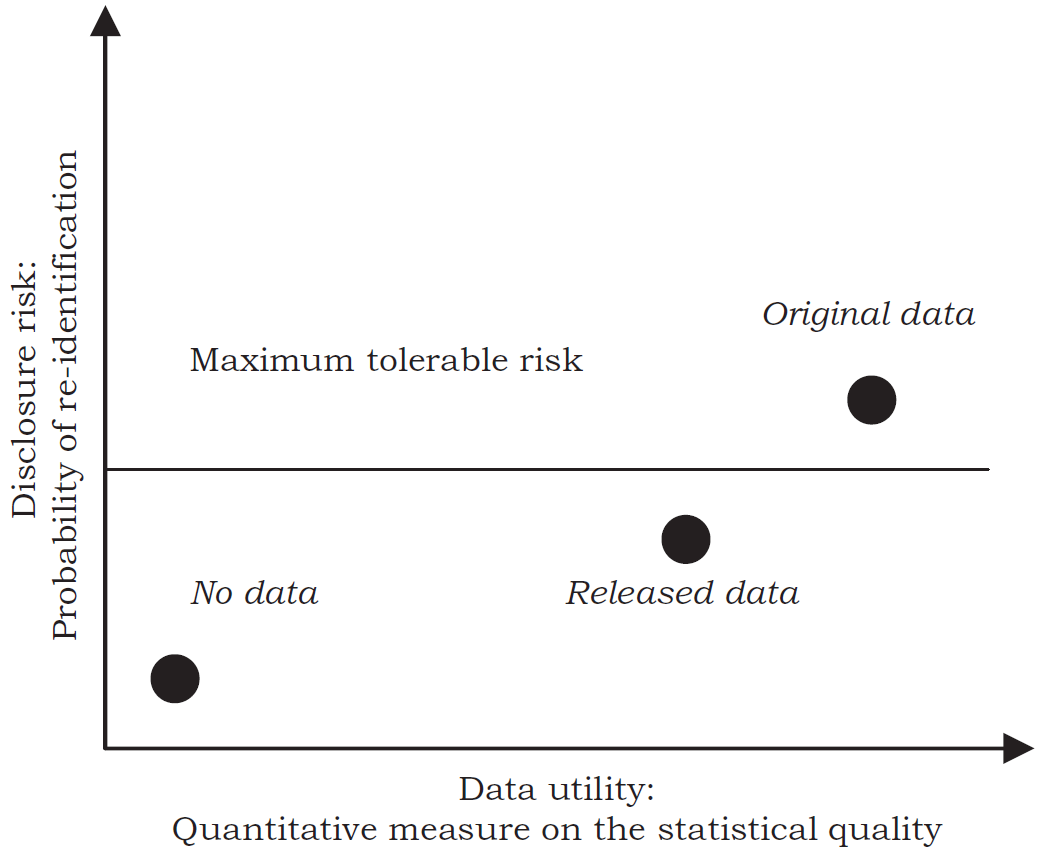
\includegraphics[width=0.55\linewidth
                    ]{Presentation//gallery/R-U confidentiality map.png}
    \caption{R-U confidentiality map (Duncan et al.,2001)}
\end{figure}

\end{frame}
% Disclosure risk %%%%%%%%%%%%%%%%%%%%%%%%%%%%%%%%%%%%%%%%%%%%%%%%%%%%%%%%%%%%%%
\begin{frame}{Disclosure risk}

A unit is at risk of disclosure when it cannot be confused with several
other units in the data set.

\begin{itemize}
\item
  \textbf{k-anonymity} A data set is said to satisfy k-anonymity for k
  \textgreater{} 1 if, for each combination of values of
  quasi-identifiers (e.g.~name, address, age, gender, etc.), at least k
  records exist in the data set sharing that combination.
\item
  Ensures that each record is indistinguishable from at least k-1 other
  records with respect to the quasi-identifiers.
\end{itemize}

More robust approaches:

\begin{itemize}
\item
  \textbf{l-Diversity} Extends k-anonymity by ensuring that the
  sensitive attribute has at least l well-represented values
\item
  \textbf{t-Closeness} Ensures that the distribution of the sensitive
  attribute in any equivalence class is close to the distribution in the
  entire dataset
\end{itemize}

\end{frame}
% Attacker Scenarios %%%%%%%%%%%%%%%%%%%%%%%%%%%%%%%%%%%%%%%%%%%%%%%%%%%%%%%%%%%
\begin{frame}{Attacker Scenarios}

\textbf{Data Intruder}: An attacker who tries to re-identify individuals
using the anonymized dataset and auxiliary information. For example,
consider a dataset of anonymized medical records. An intruder might use
publicly available information, like voter registration lists, to link
unique combinations of quasi-identifiers (such as age, gender, and zip
code) to re-identify individuals.

\textbf{Data Linkage}: This scenario involves an attacker who combines
multiple datasets to enhance the chances of re-identification. For
example, if an attacker has access to an anonymized dataset from a
hospital and another dataset from a social media platform, they might
link these datasets through common quasi-identifiers to re-identify
patients.

\textbf{Background Knowledge}: An attacker might use their own knowledge
about certain individuals to identify them in a dataset. For example, if
someone knows a particular person's age, job title, and city, they might
find a matching record in an anonymized employment dataset, thereby
re-identifying that individual.

\end{frame}
% Variables %%%%%%%%%%%%%%%%%%%%%%%%%%%%%%%%%%%%%%%%%%%%%%%%%%%%%%%%%%%%%%%%%%%%
\begin{frame}{Variables}

\begin{enumerate}
\item
  \textbf{Identifiers} - variables that can directly identify an
  individual
\item
  \textbf{Quasi-identifiers} or \textbf{key variables} - these variables
  don't identify individuals on their own but can do so when combined
  with other quasi-identifiers
\item
  \textbf{Confidential outcome variables} - variables that contain
  sensitive information that should be protected
\item
  \textbf{Non-confidential outcome variables} - these are variables that
  are not sensitive and don't risk the privacy of individuals if
  disclosed
\end{enumerate}

\end{frame}
% Disclosure control methods %%%%%%%%%%%%%%%%%%%%%%%%%%%%%%%%%%%%%%%%%%%%%%%%%%%
\begin{frame}{Disclosure control methods}

\begin{enumerate}
\tightlist
\item
  \textbf{Masking original data}

  \begin{enumerate}
  [i.]
  \tightlist
  \item
    \textbf{Non-perturbative masking} - Methods that alter data to hide
    identities without changing its actual values
  \item
    \textbf{Perturbative masking} - Methods that add noise or alter data
    values to prevent identification
  \end{enumerate}
\item
  \textbf{Generating synthetic data}

  \begin{enumerate}
  [i.]
  \tightlist
  \item
    \textbf{Parametric methods} - Techniques that use statistical models
    based on the data's distribution to generate synthetic data.
  \item
    \textbf{Non-parametric methods} Techniques that do not assume an
    underlying distribution, using methods like bootstrapping to
    generate synthetic data.
  \item
    \textbf{Generative Adversarial Networks (GANs)} Advanced machine
    learning models that generate highly realistic synthetic data by
    training two neural networks in tandem.
  \end{enumerate}
\end{enumerate}

\end{frame}
% Which method to use? %%%%%%%%%%%%%%%%%%%%%%%%%%%%%%%%%%%%%%%%%%%%%%%%%%%%%%%%%
\begin{frame}{Which method to use?}

\textbf{The SDC process depends}:
\vspace{1em}

\begin{enumerate}
    \item Type of data
        \normalsize
        \begin{itemize}
            \normalsize
            \item Full population vs Sample data
        \end{itemize}
    \item Meta information
        \begin{itemize}
            \normalsize
            \item Sampling design
            \item Response, coverage
        \end{itemize}
    \item Type of variables
        \begin{itemize}
            \normalsize
            \item Categorical vs. Continuous
        \end{itemize}
    \item Type of (required) output
        \begin{itemize}
            \normalsize
            \item Microdata files vs tabular data
        \end{itemize}
\end{enumerate}

\end{frame}
% Packages for SDC - Microdata (Unit-level data) %%%%%%%%%%%%%%%%%%%%%%%%%%%%%%%
\begin{frame}{Packages for SDC - Microdata (Unit-level data)}

\href{https://cran.r-project.org/web/packages/sdcMicro/index.html}{\color{blue}\underline{\textbf{sdcMicro}}}
can be used to anonymize data, i.e.~to create anonymized files for
public and scientific use. It implements a wide range of methods for
anonymizing categorical and continuous (key) variables. The package also
contains a graphical user interface, which is available by calling the
function sdcGUI.

\href{https://cran.r-project.org/web/packages/synthpop/index.html}{\color{blue}\underline{\textbf{synthpop}}}
using regression tree methods to simulate synthetic data from given
data. It~is suitable to produce synthetic data when the data have no
hierarchical and cluster information (such as households) as well as
when the data does not collected with a~complex sampling design.

\href{https://cran.r-project.org/web/packages/simPop/index.html}{\color{blue}\underline{\textbf{simPop}}}
using linear and robust regression methods, random forests (and many
more methods) to simulate synthetic data from given complex data. It is
also suitable to produce synthetic data when the data have hierarchical
and cluster information (such as persons in households) as well as when
the data had been collected with a complex sampling design. It makes use
of parallel computing internally.

\end{frame}
% Packages for SDC - Tabular data (Aggregated data) %%%%%%%%%%%%%%%%%%%%%%%%%%%%
\begin{frame}{Packages for SDC - Tabular data (Aggregated data)}

\href{https://cran.r-project.org/web/packages/sdcTable/index.html}{\color{blue}\underline{\textbf{sdcTable}}}
can be used to provide confidential (hierarchical) tabular data. It
includes the HITAS and the HYPERCUBE technique and uses linear
programming packages (Rglpk and lpSolveAPI) for solving (a large amount
of) linear programs.

\href{https://cran.r-project.org/web/packages/sdcSpatial/index.html}{\color{blue}\underline{\textbf{sdcSpatial}}}
can be used to smooth or/and suppress raster cells in a map. This is
useful when plotting raster-based counts on a map. sdcHierarchies
provides methods to generate, modify, import and convert nested
hierarchies that are often used when defining inputs for statistical
disclosure control methods.

\href{https://cran.r-project.org/web/packages/SmallCountRounding/index.html}{\color{blue}\underline{\textbf{SmallCountRounding}}}
can be used to protect frequency tables by rounding necessary inner
cells so that cross-classifications to be published are safe.

\href{https://cran.r-project.org/web/packages/GaussSuppression/index.html}{\color{blue}\underline{\textbf{GaussSuppression}}}
can be used to protect tables by suppression using the Gaussian
elimination secondary suppression algorithm.

\end{frame}
% Non-perturbation methods %%%%%%%%%%%%%%%%%%%%%%%%%%%%%%%%%%%%%%%%%%%%%%%%%%%%%
\begin{frame}{Non-perturbation methods}

Non-perturbative masking does not rely on distortion of the original
data but on partial suppressions or reductions of detail.

\begin{table}[ht]   
\centering  
\begin{tabular}[t]{lccc}    
\toprule    
 Method & Continuous data & Categorical data&\\ 
\midrule    
 Sampling  & & X &\\    
 Global recoding & X & X &\\    
 Top and bottom coding& X & X &\\   
 Local suppression & & X &\\    
\bottomrule 
\end{tabular}   
\caption{Non-perturbative methods vs. data types}   
\end{table}

\end{frame}
% sdcMicro %%%%%%%%%%%%%%%%%%%%%%%%%%%%%%%%%%%%%%%%%%%%%%%%%%%%%%%%%%%%%%%%%%%%%
\begin{frame}{sdcMicro}

\begin{figure}
    \centering
    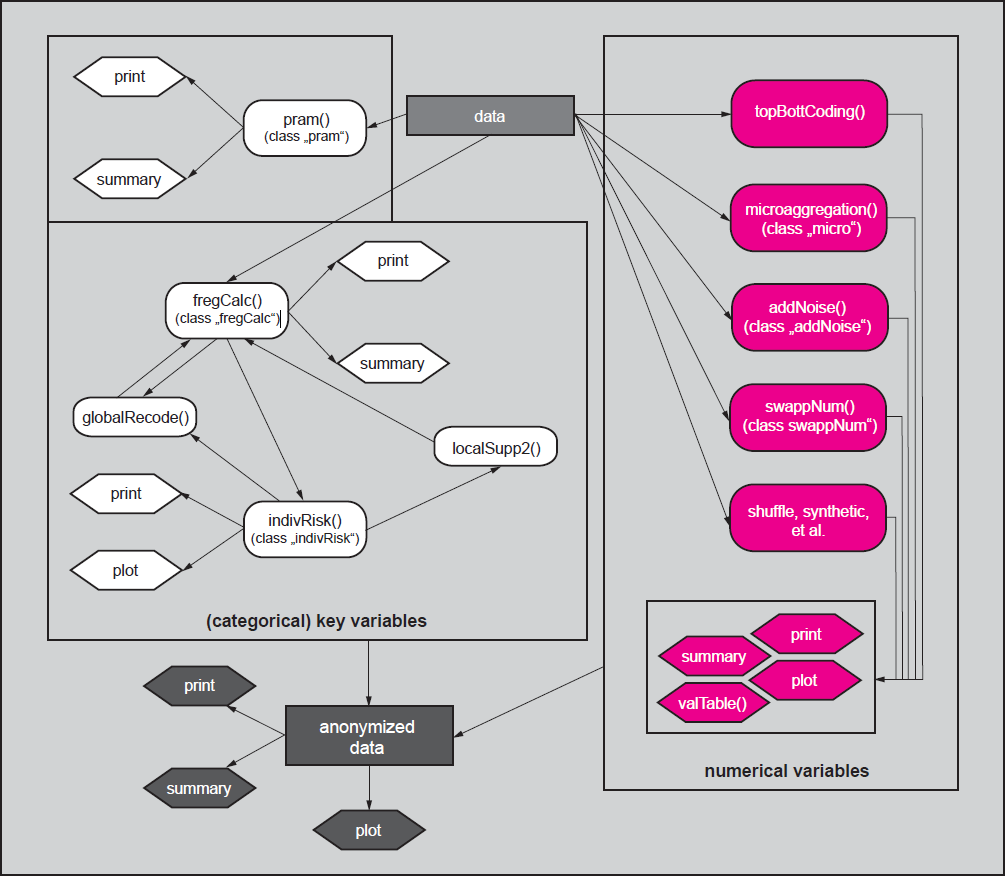
\includegraphics[width=0.5\linewidth
                    ]{Presentation//gallery/sdcMicro.png}
    \caption{Certain procedures in package \emph{sdcMicro} and their
relationship}
\end{figure}

\end{frame}
% Non-perturbation methods %%%%%%%%%%%%%%%%%%%%%%%%%%%%%%%%%%%%%%%%%%%%%%%%%%%%%
\begin{frame}{Non-perturbation methods - Example}

\begin{columns}
    \column{0.5\textwidth}
    \centering
    \Huge
    \textbf{Time to Code!}

    \column{0.5\textwidth}
    \centering
    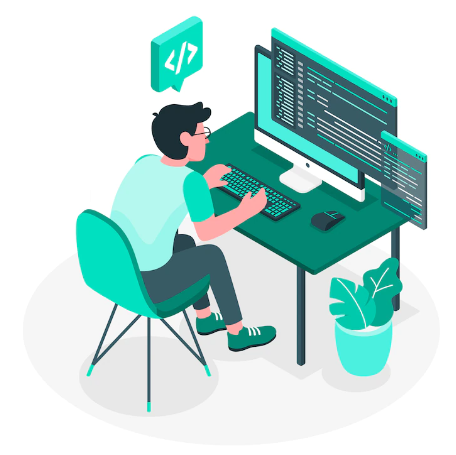
\includegraphics[width=\linewidth]{Presentation TEX//gallery/coding.png}
\end{columns}

\end{frame}
% Perturbation methods %%%%%%%%%%%%%%%%%%%%%%%%%%%%%%%%%%%%%%%%%%%%%%%%%%%%%%%%%
\begin{frame}{Perturbation methods}

This approach allows wider dissemination of data, although released are perturbed (modified) data.

There is a wide range of available methods for perturbation of data. Namely:
\vspace{1em}

\begin{itemize}
\item \textbf{Noise masking}: adding e.g. normally distributed errors \(Z = X + \varepsilon_j \sim N(0, \sigma_{\varepsilon_j}^2)\)
\item \textbf{Microaggreagtion}: grouping similar records together and replacing them with aggregate values, e.g. with their mean
\item \textbf{Record swapping}: exchanging values of specific attributes between records
\item \textbf{Rounding}: replacing original values with rounded ones
\item \textbf{Resampling}: creating multiple versions of a dataset by repeatedly drawing samples from the original data, releasing e.g. mean calculated from this samples
\item \textbf{PRAM}: probabilistically altering the values of categorical variables in a dataset according to a predefined probability matrix
  
\end{itemize}

\end{frame}
% Perturbation methods %%%%%%%%%%%%%%%%%%%%%%%%%%%%%%%%%%%%%%%%%%%%%%%%%%%%%%%%%
\begin{frame}{Perturbation methods - Example}

As the example for this approach were selected methods recommended by  
\href{https://cros.ec.europa.eu/coe-sdc}{\color{blue}\underline{\textbf{Centre of}}}
\href{https://cros.ec.europa.eu/coe-sdc}{\color{blue}\underline{\textbf{Excellence on Statistical Disclosure Control}}}
in \textbf{Harmonised protection of census data}.
\vspace{1em}

\begin{enumerate}
    \item \textbf{Target Record Swapping}
        \begin{itemize}
            \normalsize
            \item pre-tabular method applied directly to microdata
            \item selectively exchanging (swapping) values between specific pairs of records in a dataset. The pairs are chosen based on certain criteria, such as being within the same geographic area or having similar attribute values.
        \end{itemize}
    \item \textbf{Cell Key Method}
        \begin{itemize}
            \normalsize
            \item post-tabular method applied to aggregated data
            \item protect sensitive data in frequency tables
            \item adding small random noise to the cell counts
        \end{itemize}
\end{enumerate}

\end{frame}
% Target Record Swapping %%%%%%%%%%%%%%%%%%%%%%%%%%%%%%%%%%%%%%%%%%%%%%%%%%%%%%%%%%%%%
\begin{frame}{Target Record Swapping}

\centering
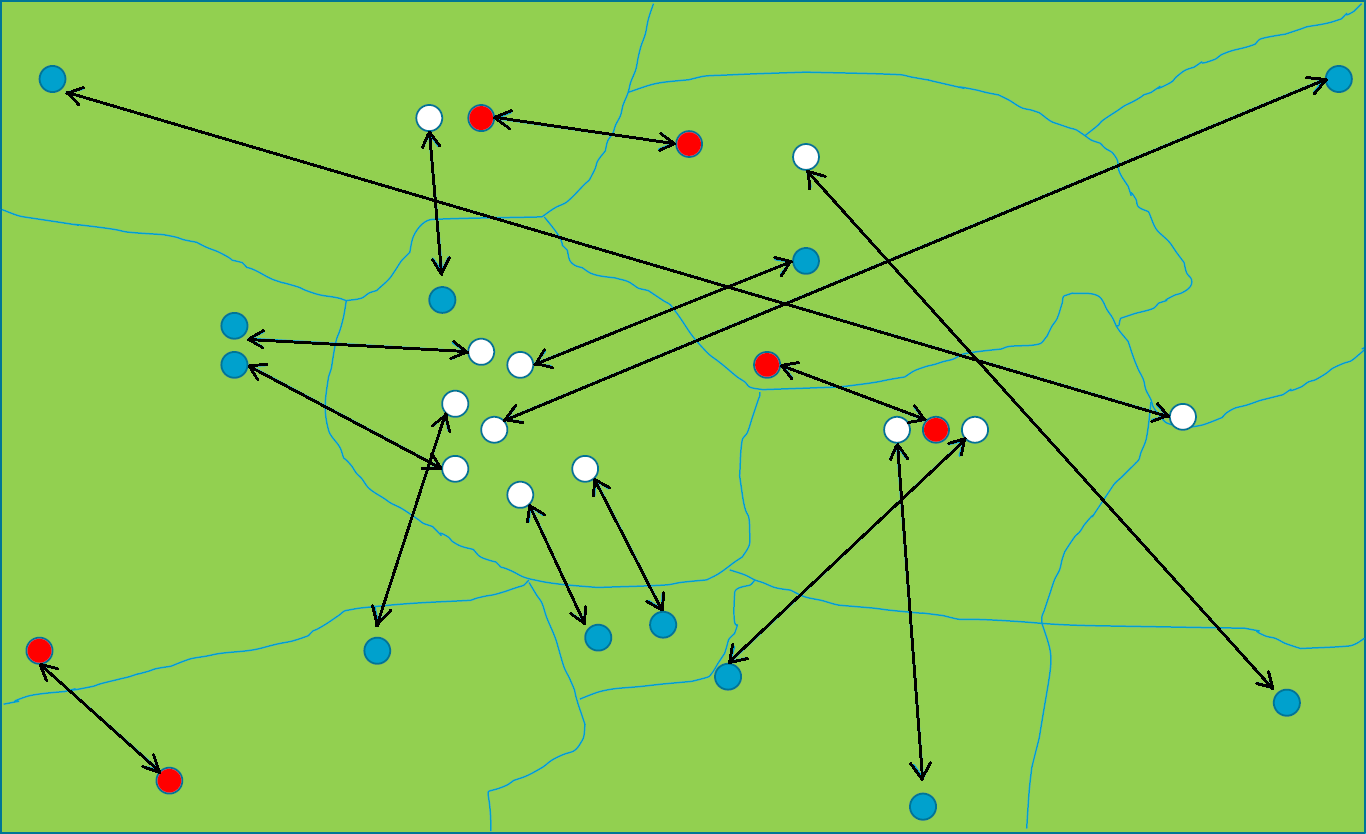
\includegraphics[width=0.8\linewidth]{Presentation TEX//gallery/record_swapping.png}

\end{frame}
% Cell Key Method %%%%%%%%%%%%%%%%%%%%%%%%%%%%%%%%%%%%%%%%%%%%%%%%%%%%%%%%%%%%%%%%%%%
\begin{frame}{Target Record Swapping}

\centering
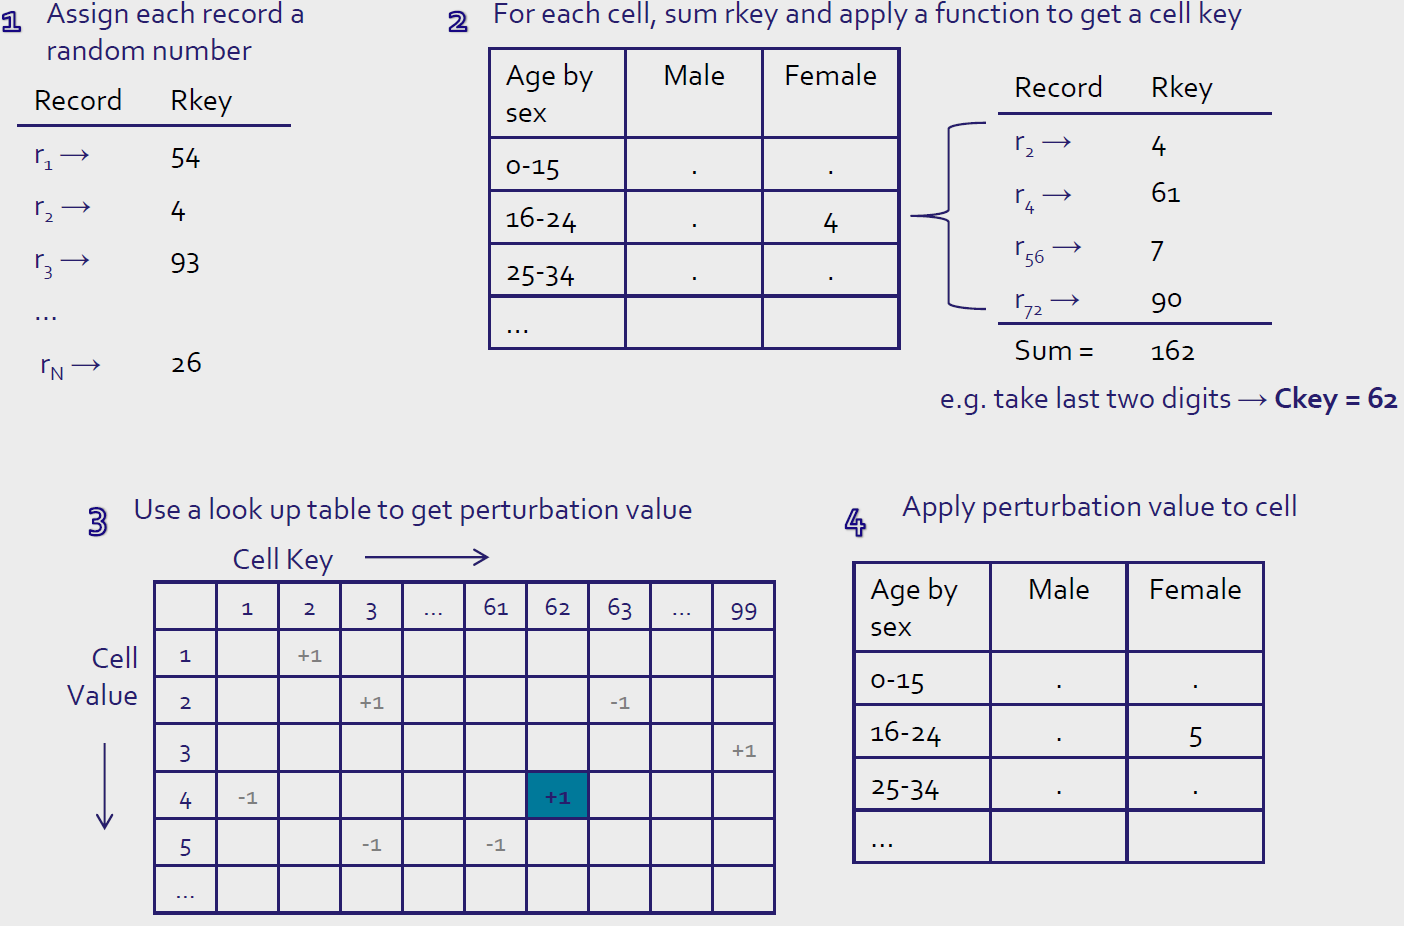
\includegraphics[width=0.8\linewidth]{Presentation TEX//gallery/cell-key.png}

\end{frame}
% Perturbation methods %%%%%%%%%%%%%%%%%%%%%%%%%%%%%%%%%%%%%%%%%%%%%%%%%%%%%%%%%%%%%%%%%%%
\begin{frame}{Perturbation methods - Example}

\begin{columns}
    \column{0.5\textwidth}
    \centering
    \Huge
    \textbf{Time to Code!}

    \column{0.5\textwidth}
    \centering
    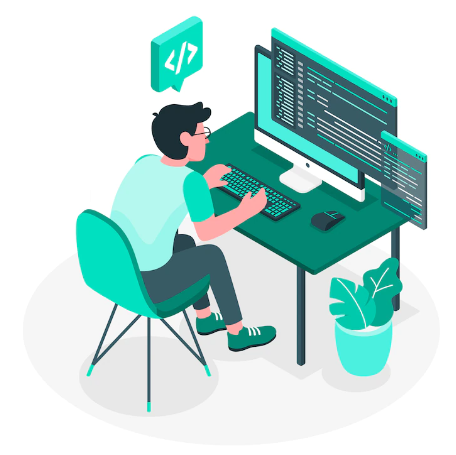
\includegraphics[width=\linewidth]{Presentation TEX//gallery/coding.png}
\end{columns}

\end{frame}
% Synthetic methods - Purpose %%%%%%%%%%%%%%%%%%%%%%%%%%%%%%%%%%%%%%%%%%%%%%%%%%%%%%%%%%%%
\begin{frame}{Synthetic methods - Purpose of Synthetic Data}

\textbf{What is Synthetic data?}
\begin{itemize}
    \item Data generated by models trained on real world data
    \item Joint and conditional/sequential models
    \begin{itemize}
    \item  Joint modeling captures entire data distribution simultaneously, powerful but computationally heavy
    \item Conditional/sequential  modeling generates data variable-by-variable based on conditional relationships, offering flexibility and scalability, but can miss intricate dependencies if not explicitly included
    \end{itemize}
    \item Preserve correlation structure (quasi-identical distribution)    
\end{itemize}

\textbf{Why generate synthetic micro data?}
\begin{itemize}
\item Demand from scientific community and public
\item GDPR and other national data protection laws often make dissemination of micro data impossible
\item Highly censored microdata
\item Long and tedious process to get access
\end{itemize}

\end{frame}
% Synthetic methods - Utility and Risk Evaluation%%%%%%%%%%%%%%%%%%%%%%%%%%%%%%%%%%%%%%%%%
\begin{frame}{Synthetic methods - Utility and Risk Evaluation}

\textbf{Utility and Risk Evaluation}

\begin{itemize}
    \item Trade-off
    \item Utility Evaluation of synthetic data \small{(many methods common to measures measuring validity of perturbated data)}
    
        \begin{itemize}
        \item Global (direct comparison on an aggregated level)
        \item Fit-for-Purpose (starting point of assessment)
        \item Outcome-Specific (for a specific analysis task)
        \end{itemize}
    \item Risk Assessment
    
\end{itemize}
\end{frame}
\begin{frame}{Synthetic methods - Utility measures }
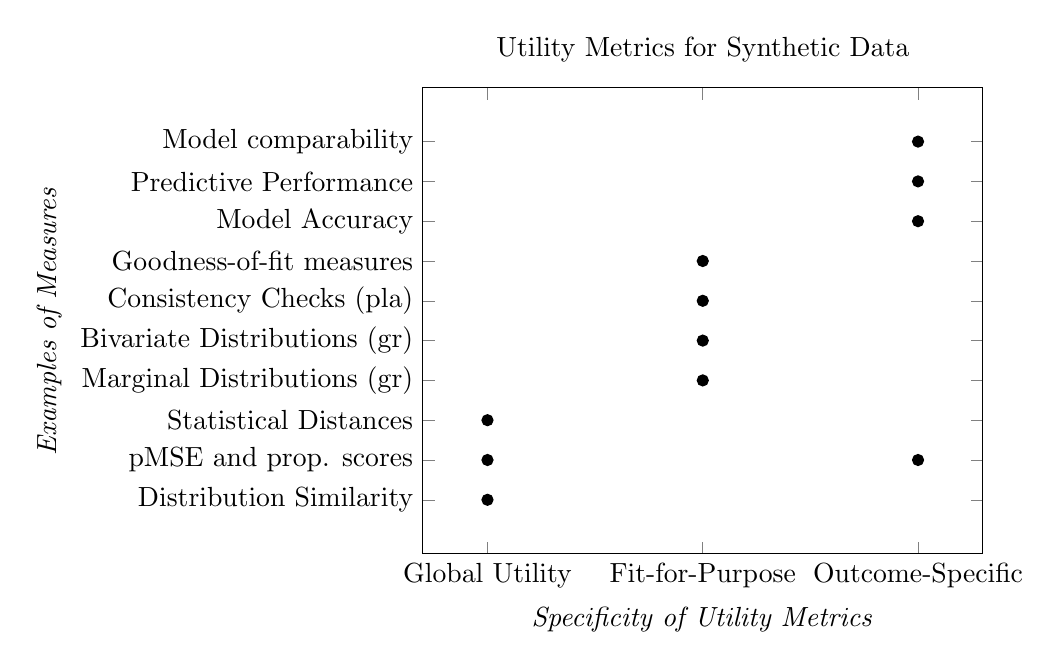
\begin{tikzpicture}
\begin{axis}[
    title={Utility Metrics for Synthetic Data},
    xlabel={\textit{Specificity of Utility Metrics}},
    ylabel={\textit{Examples of Measures}},
    xtick={1, 2, 3},
    xticklabels={Global Utility, Fit-for-Purpose\quad, Outcome-Specific},
    ytick={1, 2, 3, 4, 5, 6, 7, 8, 9, 10},
    yticklabels={
    Distribution Similarity, 
    pMSE and prop. scores, 
    Statistical Distances, 
    Marginal Distributions (gr), 
    Bivariate Distributions (gr), 
    Consistency Checks (pla), 
    %\shortstack{Goodness-of-fit measures\\\small{(e.g. Kolmogorov-Smirnov test)}},
    Goodness-of-fit measures,
    Model Accuracy, 
    Predictive Performance,
    Model comparability,
    Confidence Interval Overlap},
    enlargelimits=0.15,
    legend style={at={(0.5,-0.15)}, anchor=north,legend columns=-1},
    ylabel near ticks,
    width=8.69cm
]
\addplot[only marks, mark=*] coordinates {(1,1) (1,2) (1,3)};
\addplot[only marks, mark=*] coordinates {(2,4) (2,5) (2,6) (2,7)};
\addplot[only marks, mark=*] coordinates {(3,2) (3,8) (3,9) (3,10)};
\end{axis}
\end{tikzpicture}
\end{frame}
% Synthetic methods: Risk %%%%%%%%%%%%%%%%%%%%%%%%%%%%%%%%%%%%%%%%%%%%%%%%%%
\begin{frame}{Synthetic methods - Risk measures}
Link between original and synthetic data is broken, however this does not mean that fully synthetic
data can be assumed to have no risk of spilling sensitive information. Measuring disclosure risk for synthetic data remains challenging
\begin{itemize}
    \item Synthetic identical records with unique combination of attributes in the original data
    \item Average of distances to closest neighbours 
    \item Targeted Correct Attribution Probability (TCAP)
    \item Attack scenarios
    \begin{itemize}
    \item Membership attacks (attacker will learn that a certain record was present in the original data, e.g. Survey of Prison Inmates)
    \item Inference attacks (what an attacker can learn about unknown sensitive value after seeing the synthetic data)
    \end{itemize}
    \end{itemize}

\end{frame}
% Synthetic methods: synthpop %%%%%%%%%%%%%%%%%%%%%%%%%%%%%%%%%%%%%%%%%%%%%%%%%%
\begin{frame}{Synthetic methods: synthpop}

\textcolor{red}{Generate synthetic individual-level data without complex data structure using conditional
modeling. Parametric and non-parametric methods for SDC are available. Among the parametric methods are
included various types of regression, like normal linear, logistic, polytomous
and ordered. Non-parametric methods are based on classification and regression trees models. The package also includes a log-linear model approach for
categorical data implemented via an ipf procedure.}

\end{frame}
% Synthetic methods: synthpop %%%%%%%%%%%%%%%%%%%%%%%%%%%%%%%%%%%%%%%%%%%%%%%%%%
\begin{frame}{Synthetic methods: synthpop}

Nowok B, Raab GM, Dibben C (2016). synthpop: Bespoke Creation of
Synthetic Data in R. Journal of Statistical Software, 74(11), 1-26.
doi:10.18637/jss.v074.i11. URL
\href{https://www.jstatsoft.org/article/view/v074i11}{\color{blue}\underline{\textbf{https://www.jstatsoft.org/article/view/v074i11}}}

\end{frame}
% Synthetic methods: simPop %%%%%%%%%%%%%%%%%%%%%%%%%%%%%%%%%%%%%%%%%%%%%%%%%%%%
\begin{frame}{Synthetic methods: simPop}

Specifically designed for synthesising populations 

\begin{figure}
    \centering
    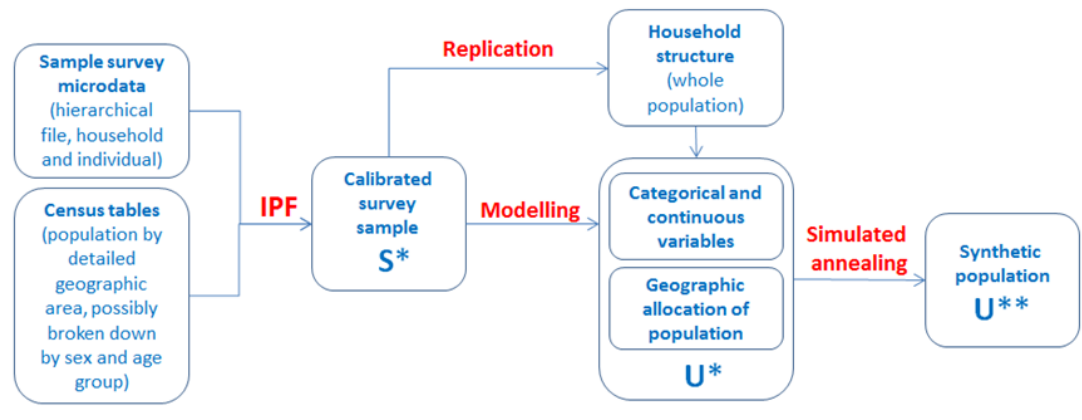
\includegraphics[width=\textwidth]{Presentation TEX/gallery/pipeline_simPop.png}
    \caption{Certain procedures in package \emph{simPop} and their
relationship}
\end{figure}

\end{frame}

% Synthetic methods: simPop %%%%%%%%%%%%%%%%%%%%%%%%%%%%%%%%%%%%%%%%%%%%%%%%%%%%
%\begin{frame}{Synthetic methods: simPop}


%Meindl B, Templ M, Alfons A, Kowarik A (2016). simPop: Simulation of
%Synthetic Populations for Survey Data Considering Auxiliary
%Information. R package version 0.3.0, URL
%\href{https://CRAN.R-project.org/package=simPop}{\color{blue}\underline{\textbf{https://CRAN.R-project.org/package=simPop}}}

%Parametric and non-parametric methods.

%\end{frame}

\begin{frame}{simPop - Example}

\begin{columns}
    \column{0.5\textwidth}
    \centering
    \Huge
    \textbf{Time to Code!}

    \column{0.5\textwidth}
    \centering
    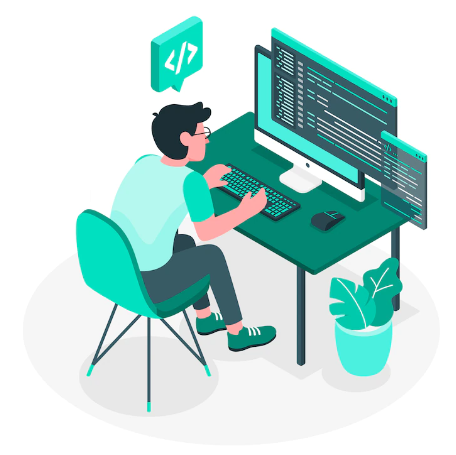
\includegraphics[width=\linewidth]{Presentation TEX//gallery/coding.png}
\end{columns}

\end{frame}

% Synthetic methods: GANs %%%%%%%%%%%%%%%%%%%%%%%%%%%%%%%%%%%%%%%%%%%%%%%%%%%%%%
\begin{frame}{Synthetic methods: GANs - Era of GANs}

	\begin{figure}[h]
		\begin{minipage}{.45\textwidth}
		  Prompt: \newline
		  An illustration of an avocado sitting in a therapist's chair, saying "I just feel so empty inside" with a pit-sized hole in its center. The therapist, a spoon, scribbles notes.
		\end{minipage}
		\begin{minipage}{.45\textwidth}
			\begin{figure}[h]
			\centering
			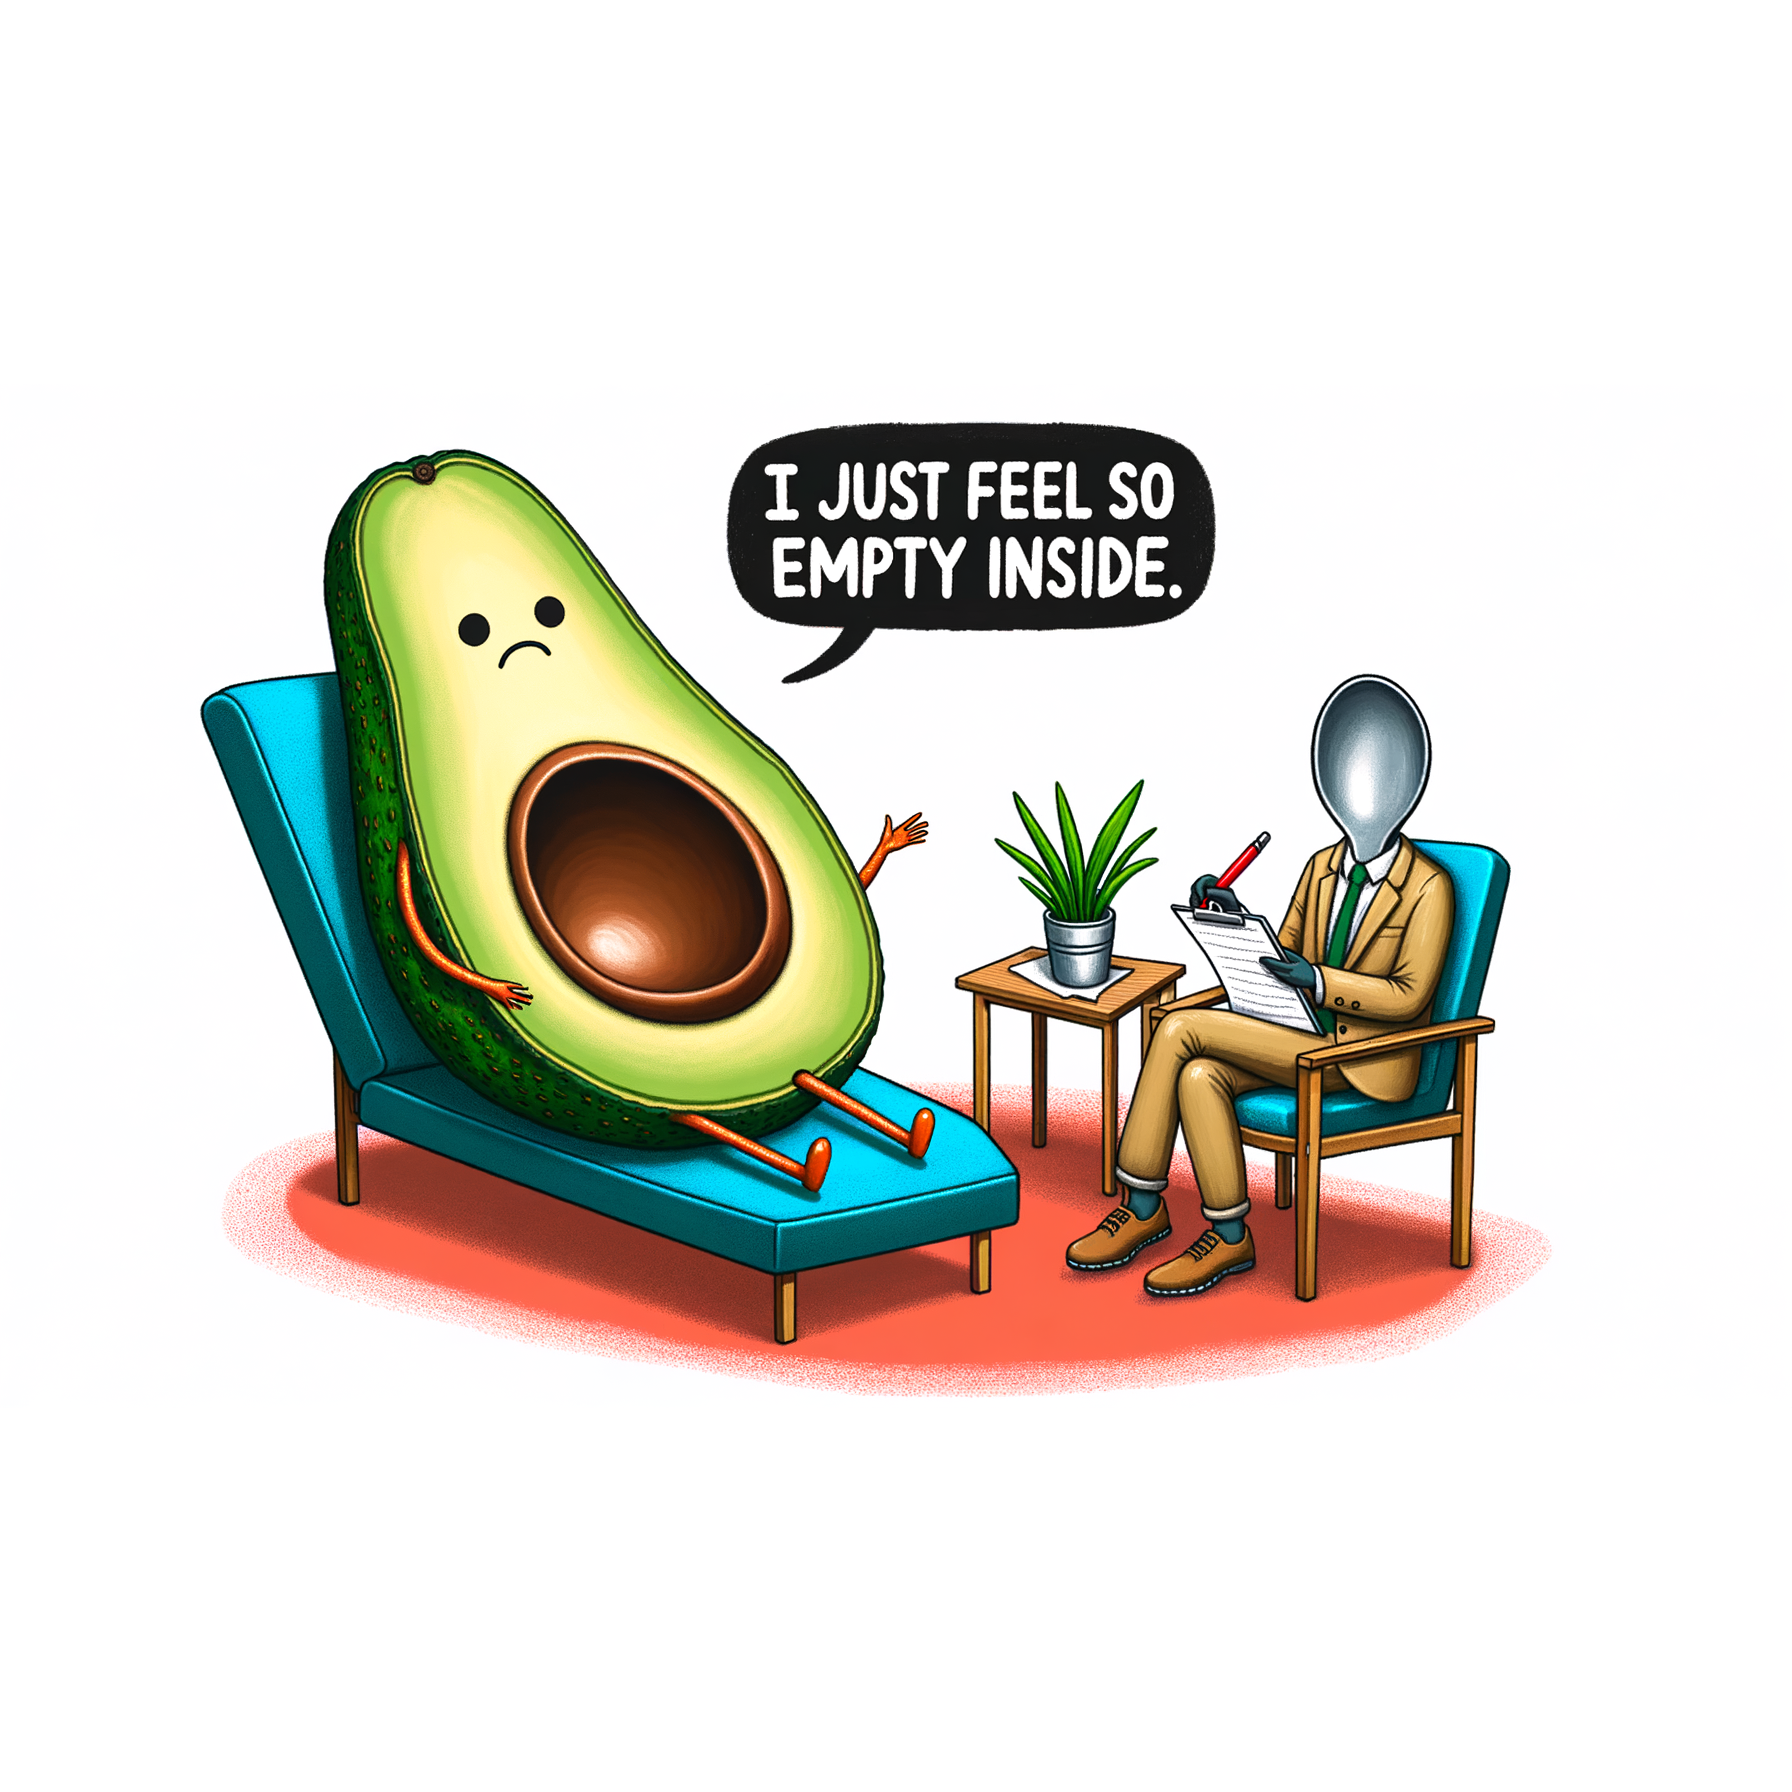
\includegraphics[width=\textwidth]{gallery/avocado-square.png}
			\vspace*{-20mm}
			\caption{Result of Text to Image}
			\end{figure}
		\end{minipage}
	\end{figure}
	\tiny{\url{https://openai.com/dall-e-3}}
 
\end{frame}
% New Slidey %%%%%%%%%%%%%%%%%%%%%%%%%%%%%%%%%%%%%%%%%%%%%%%%%%%%%%%%%%%%%%%%%%%
\begin{frame}{Synthetic methods: GANs - Overview of GAN Structure}

\begin{figure}
    \centering
    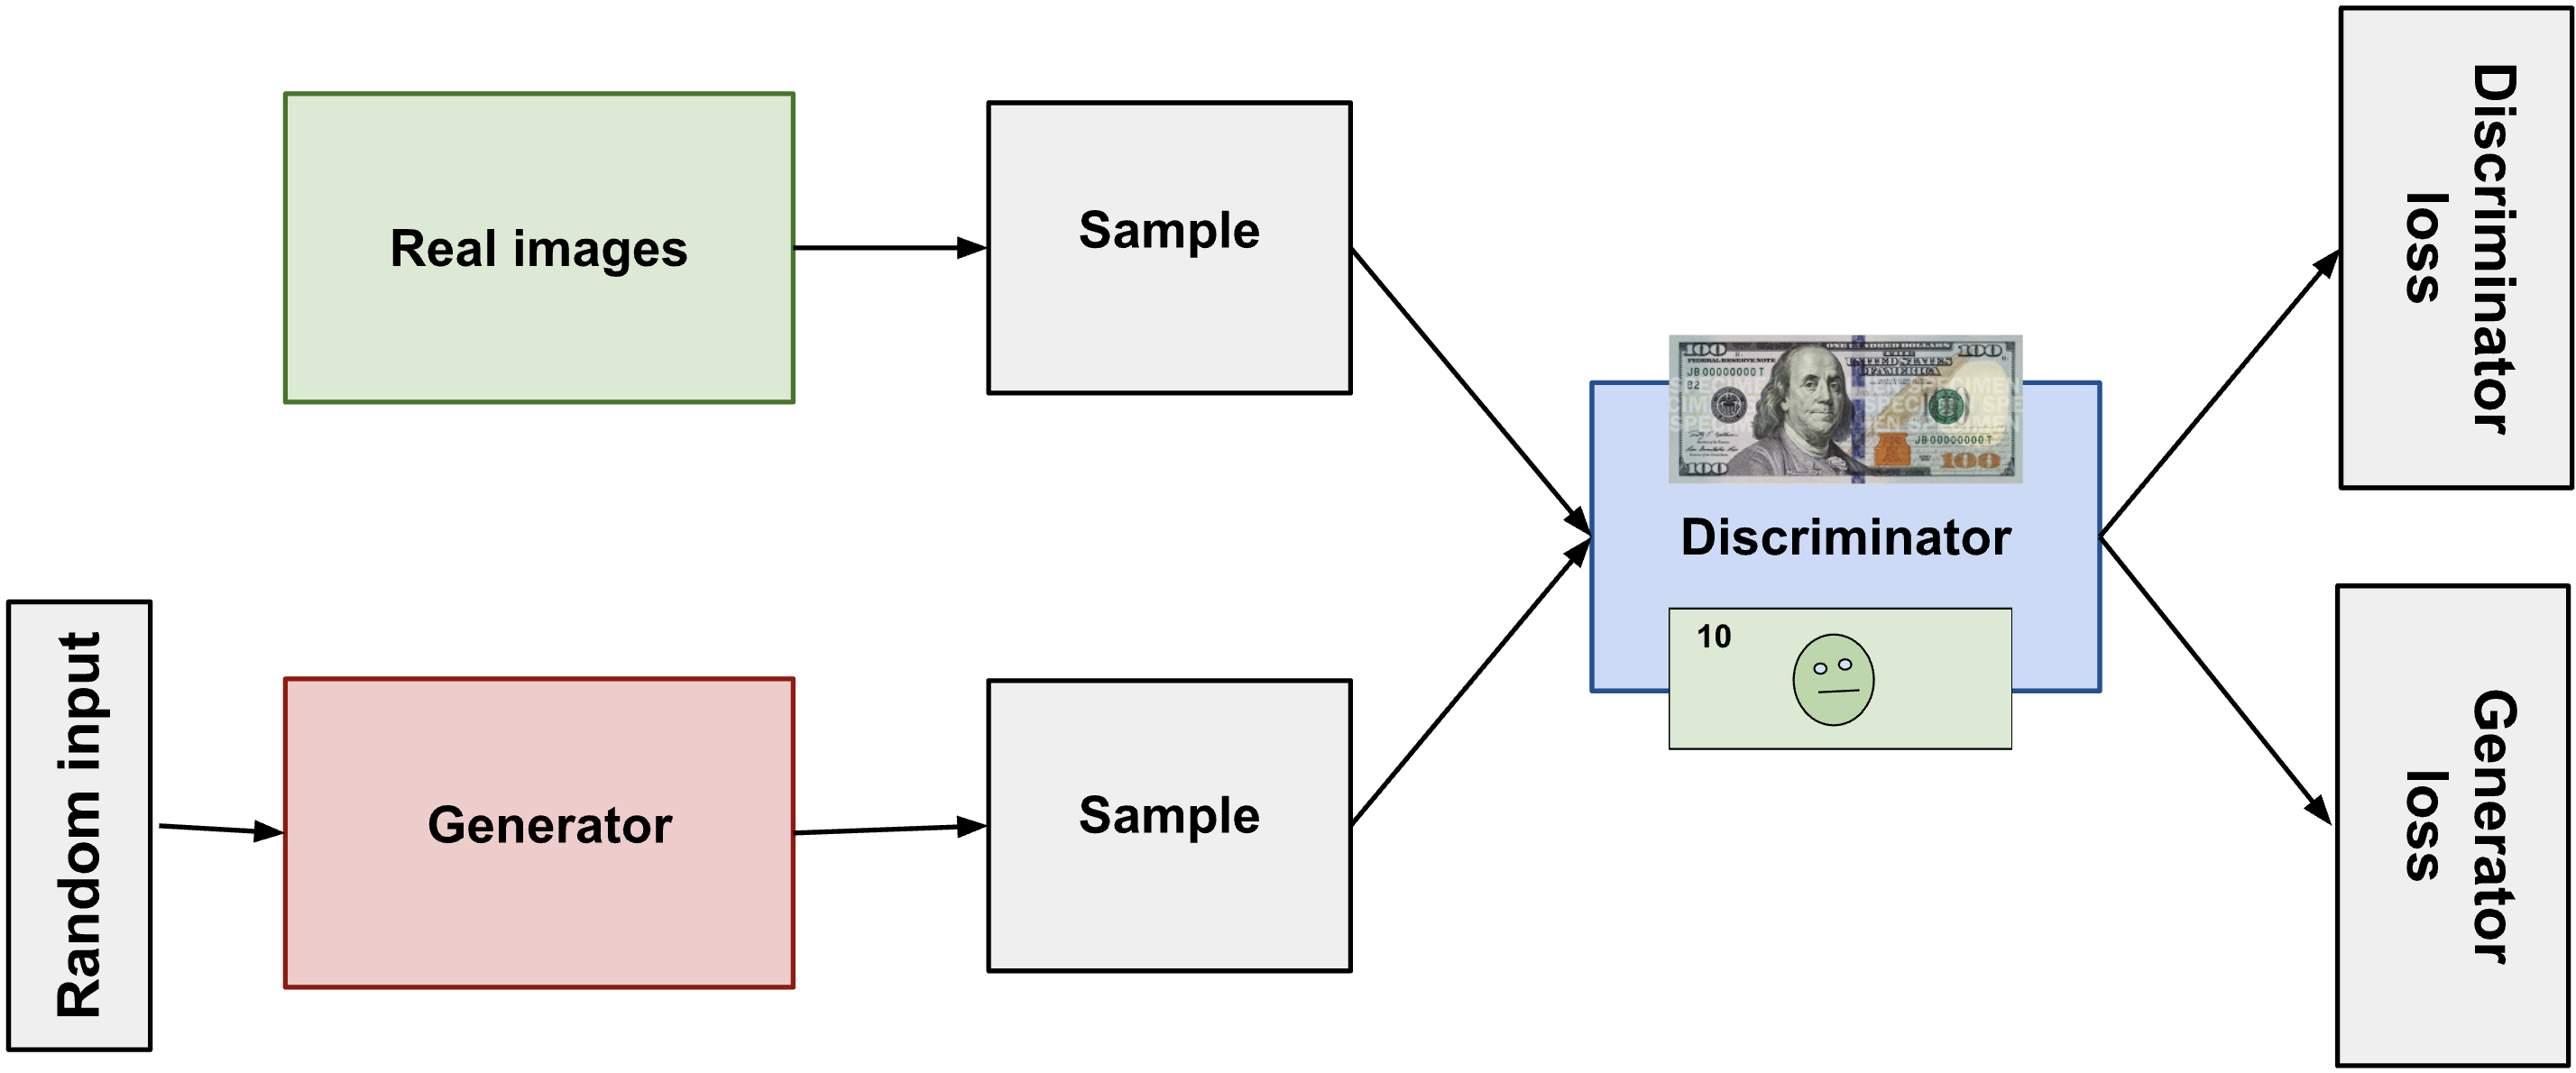
\includegraphics[width=0.9\linewidth
                    ]{gallery/gan-structure.png}
    \caption{The GAN-Framework}
\end{figure}

\end{frame}
% New Slidey %%%%%%%%%%%%%%%%%%%%%%%%%%%%%%%%%%%%%%%%%%%%%%%%%%%%%%%%%%%%%%%%%%%
\begin{frame}{Synthetic methods: GANs - Minimax Loss}

	\begin{itemize}
		\item The generator tries to minimize the following function while the discriminator tries to maximize it:
	\end{itemize}
	\[
	\mathcal{L}(G, D) = \min_G \max_D \mathbb{E}_{x \sim p_{\text{data}}(x)} [\log D(x)] + \mathbb{E}_{z \sim p_z(z)} [\log(1 - D(G(z)))]
	\]
	\begin{itemize}
		\item \(D(x)\) is the discriminator's estimate of the probability that real data instance x is real
		\item \(\mathbb{E}_x\) is the expected value over all real data instances
		\item \(G(z)\) is the generator's output when given noise z
		\item \(D(G(z))\) is the discriminator's estimate of the probability that a fake instance is real
		\item \(\mathbb{E}_z\) is the expected value over all random inputs to the generator (in effect, the expected value over all generated fake instances \(G(z)\))
	\end{itemize}
	\vspace{5mm}
	\tiny{\url{https://developers.google.com/machine-learning/gan/loss}}
 
\end{frame}
% New Slidey %%%%%%%%%%%%%%%%%%%%%%%%%%%%%%%%%%%%%%%%%%%%%%%%%%%%%%%%%%%%%%%%%%%
\begin{frame}{Synthetic methods: GANs - CTGAN: Conditional Tabular GAN for Tabular Data Synthesis}
   
    \begin{itemize}
        \item \textbf{Purpose}: Generate realistic synthetic tabular data.
        \item \textbf{Core Idea}: Uses GANs to capture the distribution of tabular data, including complex relationships between features.
        \item \textbf{Advantages}:
        \begin{itemize}
            \item Handles mixed data types (continuous and categorical).
            \item Captures complex dependencies in the data.
            \item Useful for data augmentation, privacy preservation, and data sharing.
        \end{itemize}
    \end{itemize}
    
\end{frame}
% New Slidey %%%%%%%%%%%%%%%%%%%%%%%%%%%%%%%%%%%%%%%%%%%%%%%%%%%%%%%%%%%%%%%%%%%
\begin{frame}{Synthetic methods: GANs - CTGAN: Why use it?}
 
  \begin{figure}
      \centering
      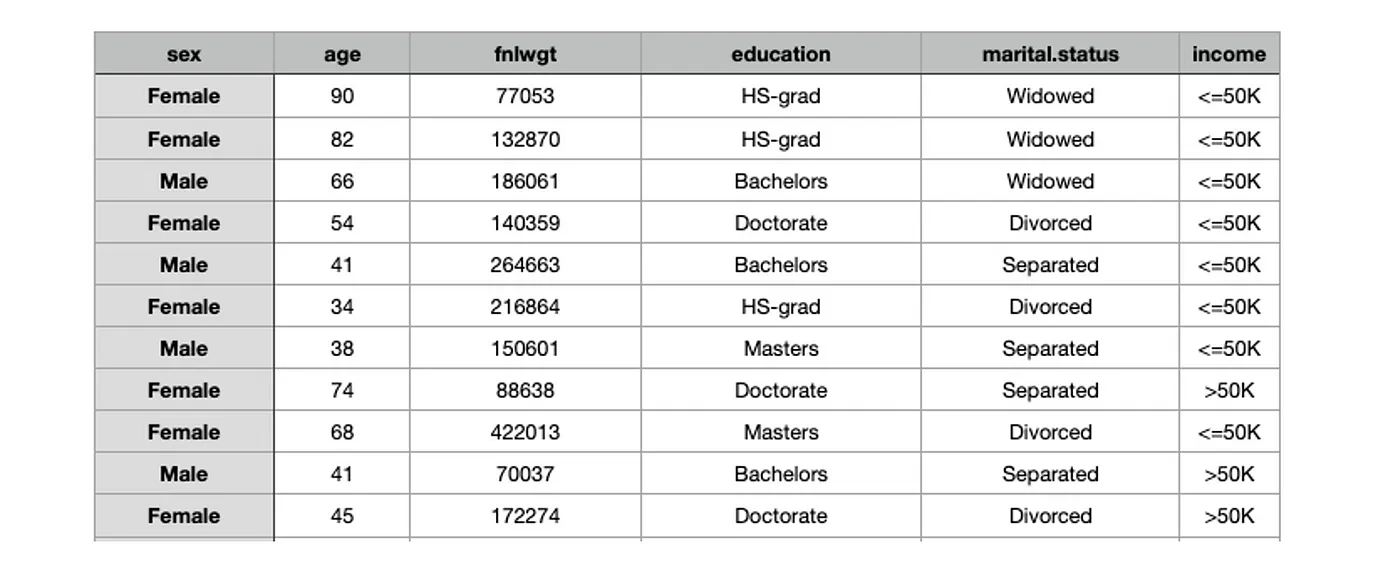
\includegraphics[width=0.5\linewidth]{Presentation TEX/gallery/table.png}
  \caption{Heterogeneous Tabular Data}
  \end{figure}
  CTGAN was developed to deal with the challenges posed by tabular datasets, handling mixed data types (numeric and categorical).
  \begin{enumerate}
      \item Other GANs, e.g., \href{https://pubmed.ncbi.nlm.nih.gov/32167919/}{\color{blue}\underline{ADS-GAN}} that use Wasserstein GAN with Gradient Penalty, in order to improve training stability and convergence time, aren't able to handle mixed data types.
  \end{enumerate}
  \vspace{2.5mm}
\tiny{\url{https://miro.medium.com/v2/resize:fit:1400/format:webp/1*GnQJiD9-jAz9dR8vKP4Thg.png}}

\end{frame}
% New Slidey %%%%%%%%%%%%%%%%%%%%%%%%%%%%%%%%%%%%%%%%%%%%%%%%%%%%%%%%%%%%%%%%%%%
\begin{frame}{Synthetic methods: GANs - CTGAN: How does it work?}
  
  \begin{figure}
      \centering
      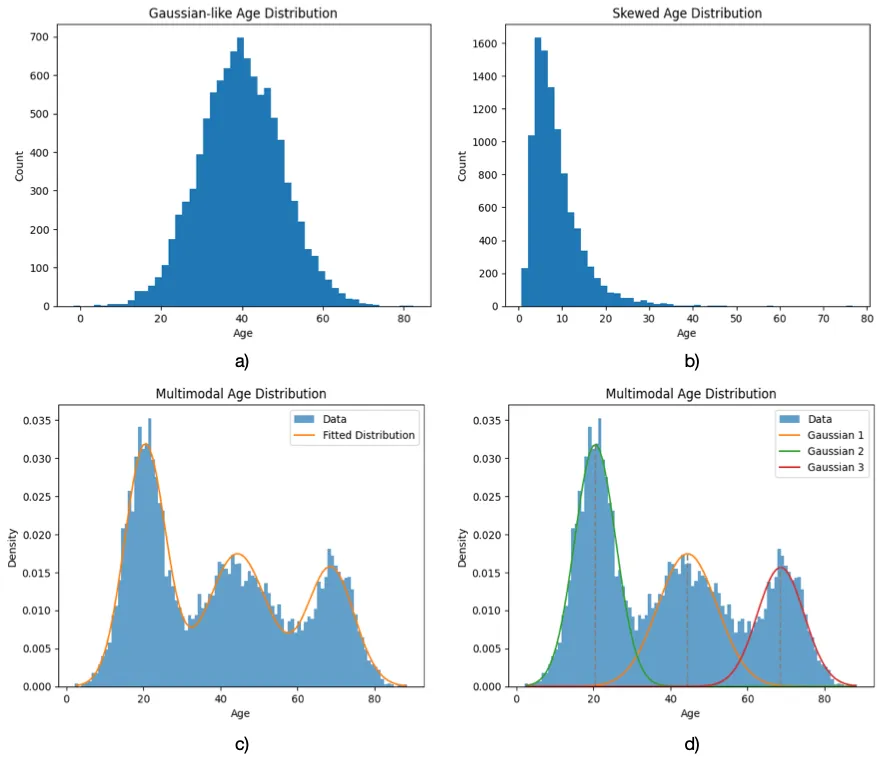
\includegraphics[width=0.3\linewidth]{Presentation TEX/gallery/gaussian-nongaussian.png}
  \caption{Heterogeneous Tabular Data: Gaussian like versus skewed data distribution (fig. a \& b). Multimodal distribution decomposed into distributions with distinct modes (fig. c \& d).}
  \end{figure}
Numerical Data in tabular data are often non-Gaussian.
\begin{enumerate}
    \item CTGAN therefore uses VGM (Variational Gaussian Mixture) model for mode-specific normalization
\end{enumerate}
\tiny{\url{https://arxiv.org/pdf/1907.00503}}
\newline
\tiny{\url{https://iopscience.iop.org/article/10.1088/1757-899X/1294/1/012024}}

\end{frame}
% New Slidey %%%%%%%%%%%%%%%%%%%%%%%%%%%%%%%%%%%%%%%%%%%%%%%%%%%%%%%%%%%%%%%%%%%
\begin{frame}{Synthetic methods: GANs - CTGAN: How does it work?}
 
  \begin{figure}
      \centering
      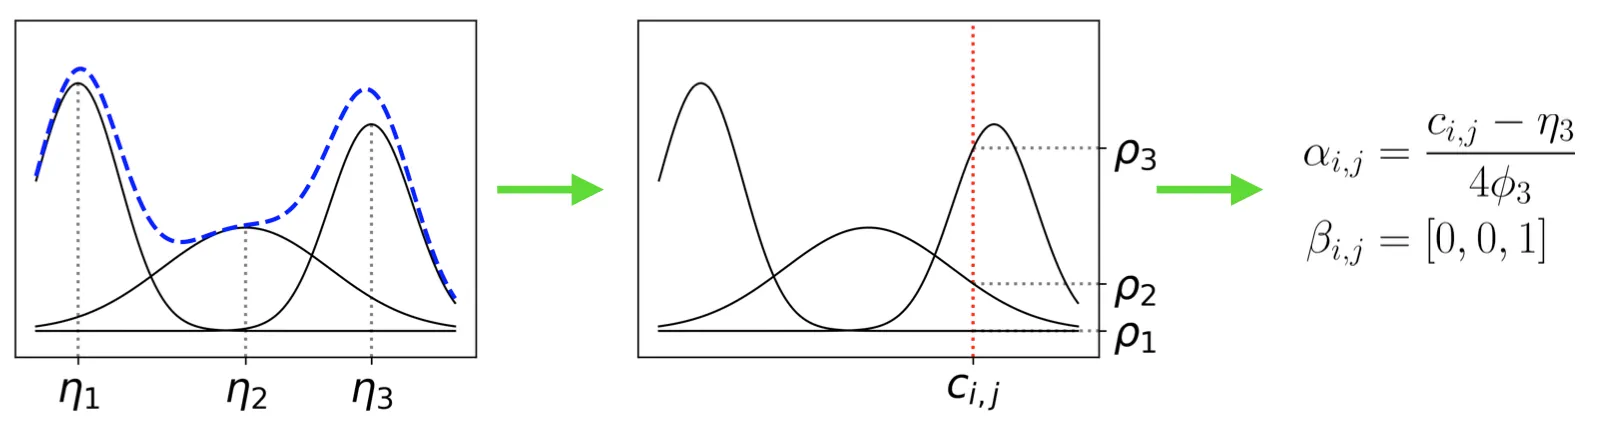
\includegraphics[width=0.5\linewidth]{Presentation TEX/gallery/mode-specific-normalization.png}
  \caption{Example of mode-specific normalization}
  \end{figure}
Using a VGM (Variational
Gaussian Mixture) model, each value in a continuous feature is represented by a one-hot vector
indicating its sampled mode and a scalar that represents the value normalized according to that mode
\vspace{2.5mm}
\newline
\tiny{\url{https://arxiv.org/pdf/1907.00503}}
\newline
\tiny{\url{https://iopscience.iop.org/article/10.1088/1757-899X/1294/1/012024}}

\end{frame}
% New Slidey %%%%%%%%%%%%%%%%%%%%%%%%%%%%%%%%%%%%%%%%%%%%%%%%%%%%%%%%%%%%%%%%%%%
\begin{frame}{Synthetic methods: GANs - CTGAN: How does it work?}
     
      \begin{figure}
      \centering
      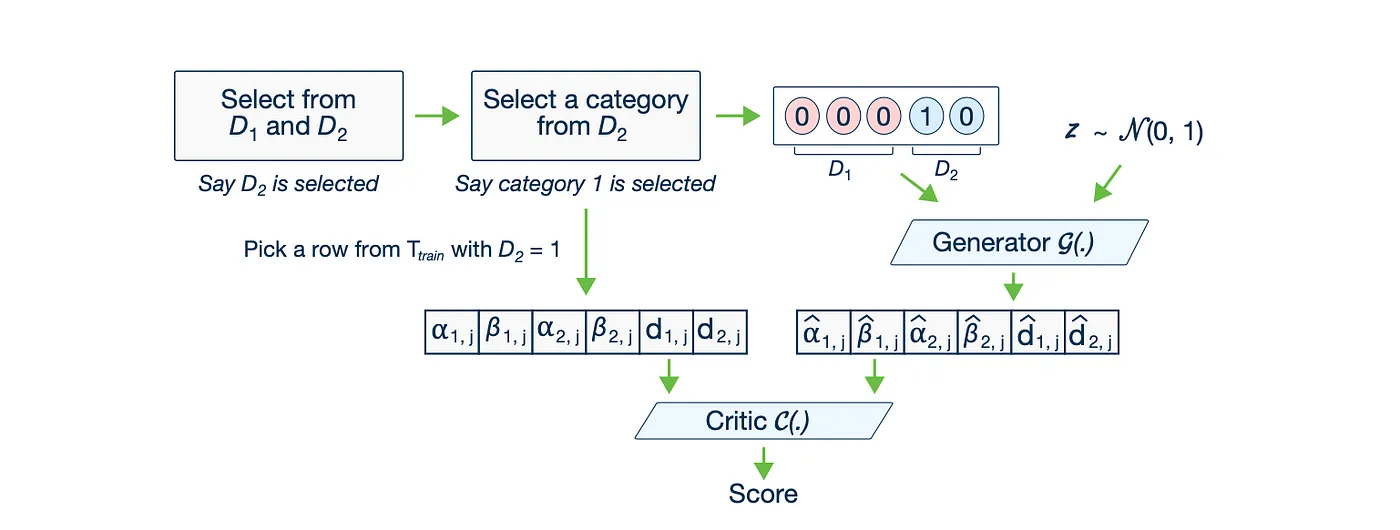
\includegraphics[width=0.6\linewidth]{Presentation TEX/gallery/training-by-sampling.png}
  \caption{Training-by-sampling in the CTGAN model}
  \end{figure}
      Input:
    \begin{itemize}
        \item Conditional vector specifying desired attributes. Noise vector from a standard normal distribution.
        \item With training-by-sampling, examples are conditioned on the possible values of categorical features, sampled according to their log-frequency. 
    \end{itemize}
\vspace{2.5mm}
\newline
\tiny{\url{https://arxiv.org/pdf/1907.00503}}
\newline
\tiny{\url{https://iopscience.iop.org/article/10.1088/1757-899X/1294/1/012024}}

\end{frame}
% New Slidey %%%%%%%%%%%%%%%%%%%%%%%%%%%%%%%%%%%%%%%%%%%%%%%%%%%%%%%%%%%%%%%%%%%
\begin{frame}{Synthetic methods: GANs - CTGAN: How does it work?}

      \begin{figure}
      \centering
      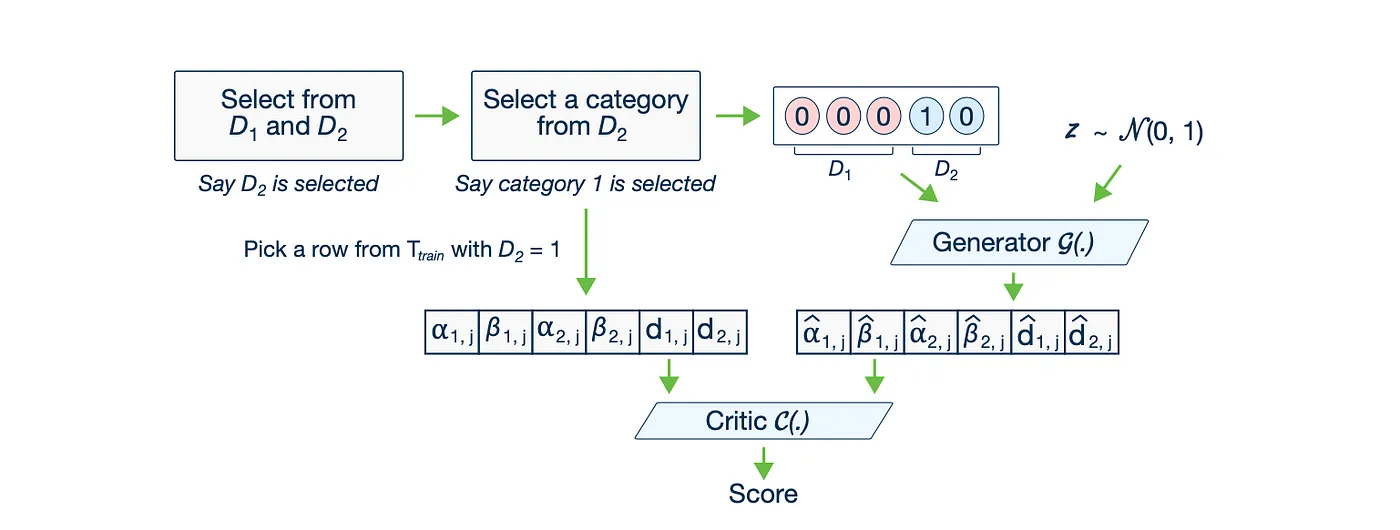
\includegraphics[width=0.6\linewidth]{Presentation TEX/gallery/training-by-sampling.png}
  \caption{Training-by-sampling in the CTGAN model}
  \end{figure}
      Conditional Vector Encoding:
    \begin{itemize}
        \item One-hot encoding for categorical columns.
        \item Gaussian Mixture Models (GMM) for continuous columns.
    \end{itemize}
\vspace{2.5mm}
\newline
\tiny{\url{https://arxiv.org/pdf/1907.00503}}
\newline
\tiny{\url{https://iopscience.iop.org/article/10.1088/1757-899X/1294/1/012024}}

\end{frame}
% New Slidey %%%%%%%%%%%%%%%%%%%%%%%%%%%%%%%%%%%%%%%%%%%%%%%%%%%%%%%%%%%%%%%%%%%
\begin{frame}{Synthetic methods: GANs - CTGAN: How does it work?}

      \begin{figure}
      \centering
      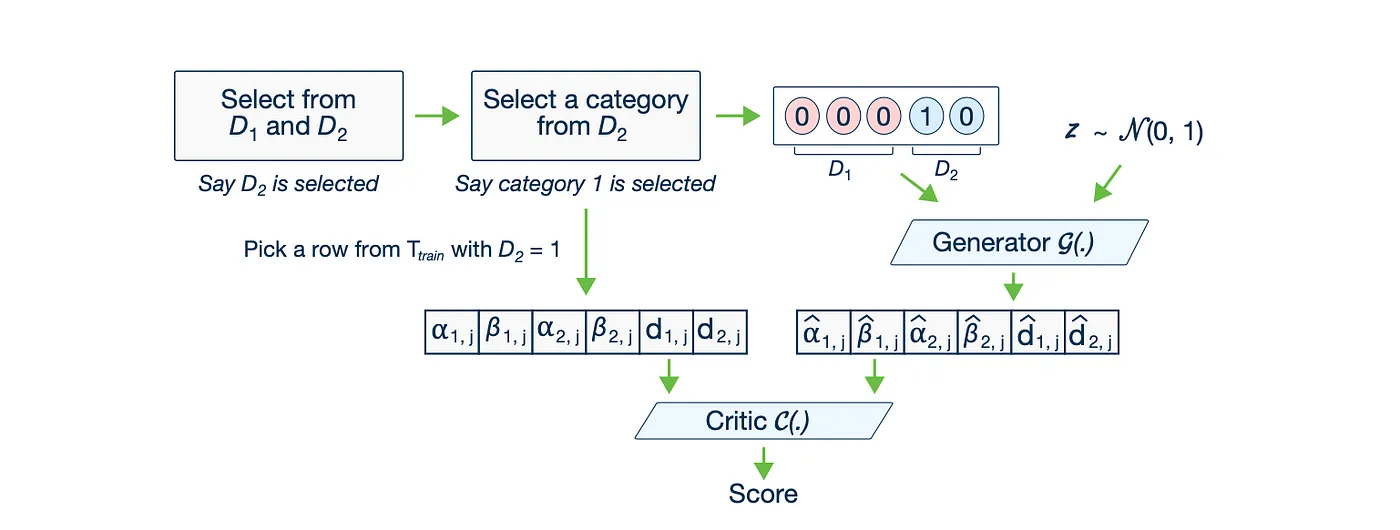
\includegraphics[width=0.6\linewidth]{Presentation TEX/gallery/training-by-sampling.png}
  \caption{Training-by-sampling in the CTGAN model}
  \end{figure}
    Generator Network:
    \begin{itemize}
        \item Neural network processes the combined input vector.
        \item Outputs a synthetic sample.
    \end{itemize}
\vspace{2.5mm}
\newline
\tiny{\url{https://arxiv.org/pdf/1907.00503}}
\newline
\tiny{\url{https://iopscience.iop.org/article/10.1088/1757-899X/1294/1/012024}}

\end{frame}
% New Slidey %%%%%%%%%%%%%%%%%%%%%%%%%%%%%%%%%%%%%%%%%%%%%%%%%%%%%%%%%%%%%%%%%%%
\begin{frame}{Synthetic methods: GANs - CTGAN: How does it work?}

      \begin{figure}
      \centering
      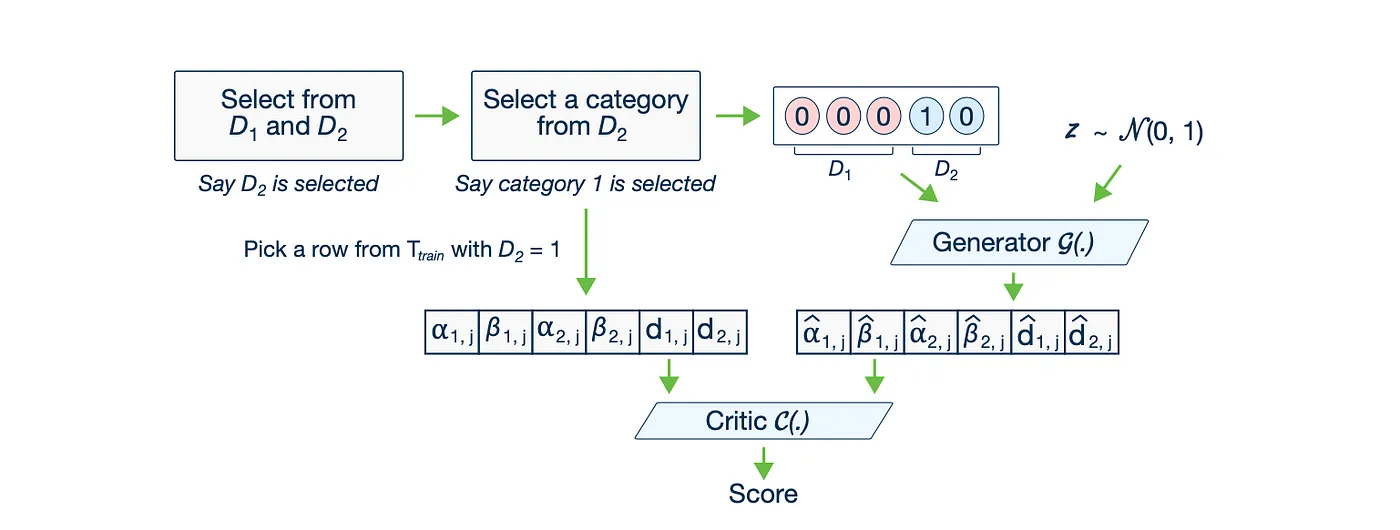
\includegraphics[width=0.6\linewidth]{Presentation TEX/gallery/training-by-sampling.png}
  \caption{Training-by-sampling in the CTGAN model}
  \end{figure}
    Training:
    \begin{itemize}
       \item Discriminator provides feedback to improve generation and the generator adjusts the synthetic data to match the conditional distribution of the specified column values, ensuring the generated data is representative of the real conditional relationships.
    \end{itemize}
\vspace{2.5mm}
\newline
\tiny{\url{https://arxiv.org/pdf/1907.00503}}
\newline
\tiny{\url{https://iopscience.iop.org/article/10.1088/1757-899X/1294/1/012024}}

\end{frame}
% New Slidey %%%%%%%%%%%%%%%%%%%%%%%%%%%%%%%%%%%%%%%%%%%%%%%%%%%%%%%%%%%%%%%%%%%
\begin{frame}{Synthetic methods: GANs - R Interface for CTGAN}

    \textbf{R Interface for CTGAN:} A wrapper around CTGAN that brings the functionalities to R users. More details can be found in the corresponding repository: \href{https://github.com/kasaai/ctgan}{\color{blue}\underline{https://github.com/kasaai/ctgan}}.
    \begin{itemize}
    \item R Interface is obsolete (code was last updated 4 years ago).
    \item Problems with installation.
    \item Problems with passing of parameters (CTGAN has seen several changes and refactoring).
    \end{itemize}

\end{frame}
% New Slidey %%%%%%%%%%%%%%%%%%%%%%%%%%%%%%%%%%%%%%%%%%%%%%%%%%%%%%%%%%%%%%%%%%%
\begin{frame}{Synthetic methods: GANs - Python Interface for CTGAN}

    \textbf{Python Interface for CTGAN:} CTGAN is a collection of Deep Learning based synthetic data generators for single table data, which are able to learn from real data and generate synthetic data with high fidelity.
    \begin{itemize}
    \item Use CTGAN through the SDV library: \href{https://github.com/sdv-dev/SDV}{\color{blue}\underline{https://github.com/sdv-dev/SDV}}
        \begin{enumerate}
           \item Preprocessing: \href{https://docs.sdv.dev/sdv/single-table-data/data-preparation}{\color{blue}\underline{Data Preparation}}
           \item Modelling: \href{https://docs.sdv.dev/sdv/single-table-data/modeling/synthesizers/ctgansynthesizer}{\color{blue}\underline{CTGANSynthesizer}}
           \item Sampling: \href{https://docs.sdv.dev/sdv/single-table-data/sampling/sample-realistic-data}{\color{blue}\underline{Sample Realistic Data}}
        \end{enumerate}
    \item Use the CTGAN standalone library: \href{https://github.com/sdv-dev/CTGAN}{\color{blue}\underline{https://github.com/sdv-dev/CTGAN}}
            \begin{enumerate}
                \item When using the CTGAN library directly, you may need to manually preprocess your data into the correct format, for example:
                \begin{enumerate}
                    \item Continuous data must be represented as floats
                    \item Discrete data must be represented as ints or strings
                    \item The data should not contain any missing values
                \end{enumerate}
        \end{enumerate}
    \end{itemize}

\end{frame}
% Last slide %%%%%%%%%%%%%%%%%%%%%%%%%%%%%%%%%%%%%%%%%%%%%%%%%%%%%%%%%%%%%%%%%%%
\begin{frame}[plain]

\centering
\Huge Thank you for your attention\\

  \vspace{2em}

  \begin{figure}
      \centering
      
\includegraphics[width=0.5\linewidth]{style/SwissAnon.png}
  \end{figure}

\large Swiss Data Anonymization Competence Center

\href{https://swissanon.ch}{\color{blue}\underline{https://swissanon.ch}}
\end{frame}

%%%%%%%%%%%%%%%%%%%%%%%%%%%%%%%%%%%%%%%%%%%%%%%%%%%%%%%%%%%%%%%%%%%%%%%%%%%%%%%%
\end{document} 

%%%%%%%%%%%%%%%%%%%%%%%%%%%%%%%%%%%%%%%%%%%%%%%%%%%%%%%%%%%%%%%%%%%%%%%%%%%%%%%%
%%%%%%%%%%%%%%%%%%%%%%%%%%%%%%%%%%%%%%%%%%%%%%%%%%%%%%%%%%%%%%%%%%%%%%%%%%%%%%%%
%%%%%%%%%%%%%%%%%%%%%%%%%%%%%%%%%%%%%%%%%%%%%%%%%%%%%%%%%%%%%%%%%%%%%%%%%%%%%%%%